\chapter{Temporal winner-loser networks}

\section{Network size evolution}\label{app:temp_network}

\begin{figure}[h!t]
    \centering

    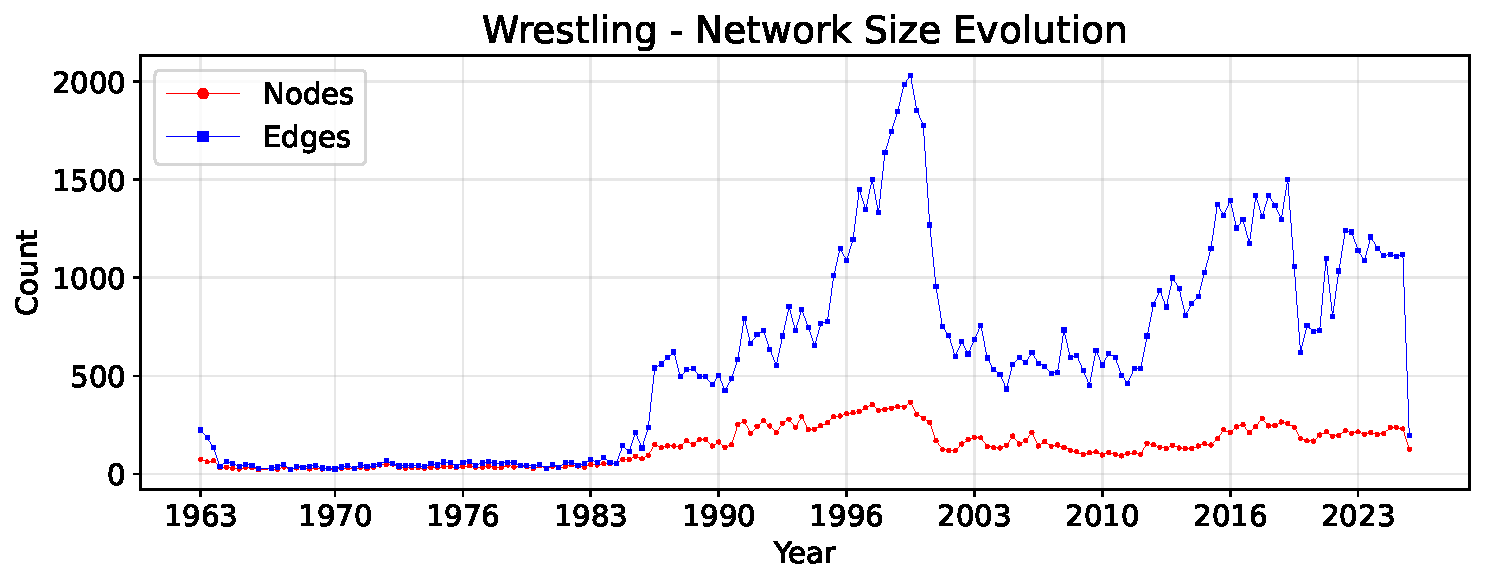
\includegraphics[width=0.8\textwidth]{plots/Wrestling_network_size_evolution.pdf}
    \vspace{0.0cm}
    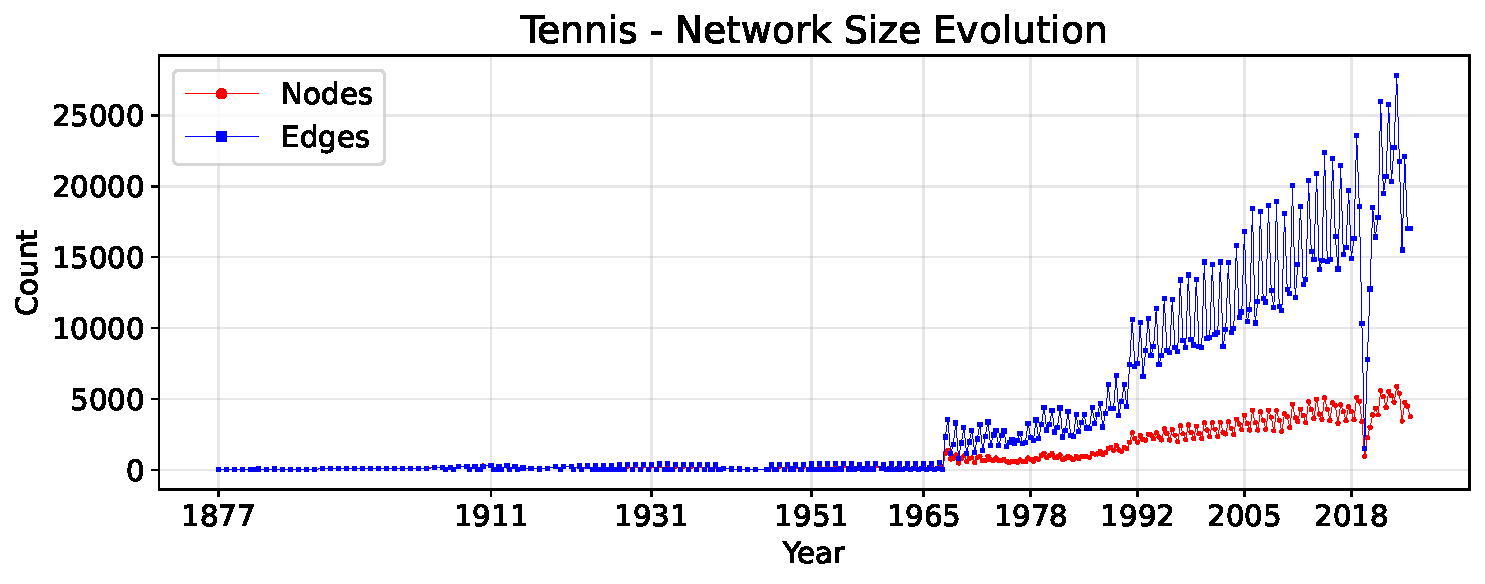
\includegraphics[width=0.8\textwidth]{plots/Tennis_network_size_evolution.pdf}
    \vspace{0.0cm}
    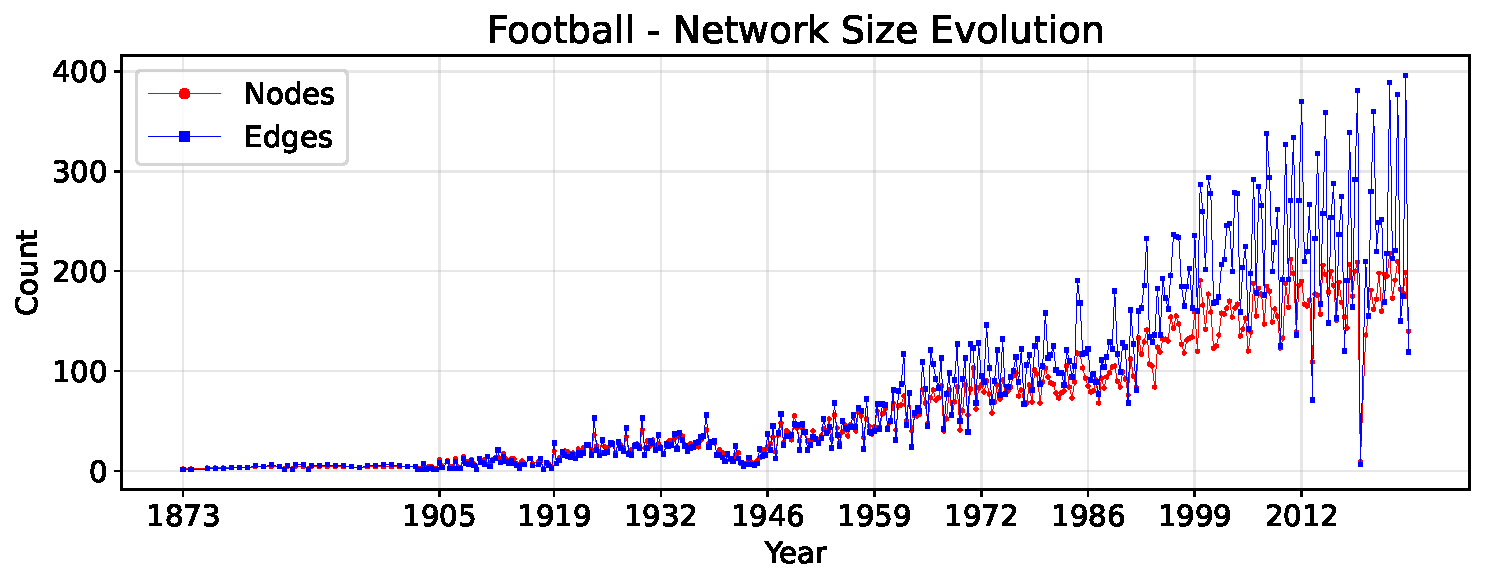
\includegraphics[width=0.8\textwidth]{plots/Football_network_size_evolution.pdf}

    \caption{Evolution of the number of nodes and edges across temporal snapshots for the Wrestling, Tennis, and Football datasets.}
    \label{fig:network_size_evolution}
\end{figure}


\clearpage
\section{Temporal evolution of structural network properties}\label{app:den_com_cen}

\begin{figure}[h!t]
    \centering

    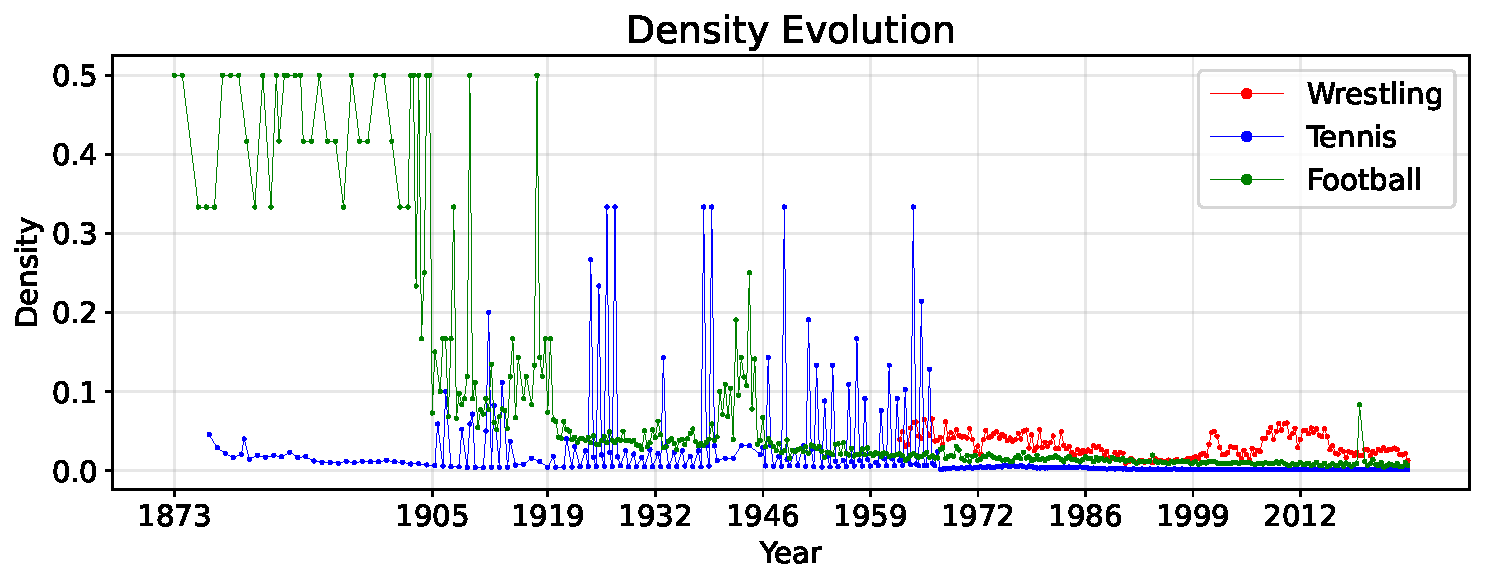
\includegraphics[width=0.8\textwidth]{plots/density_comparison.pdf}
    \vspace{0.0cm}
    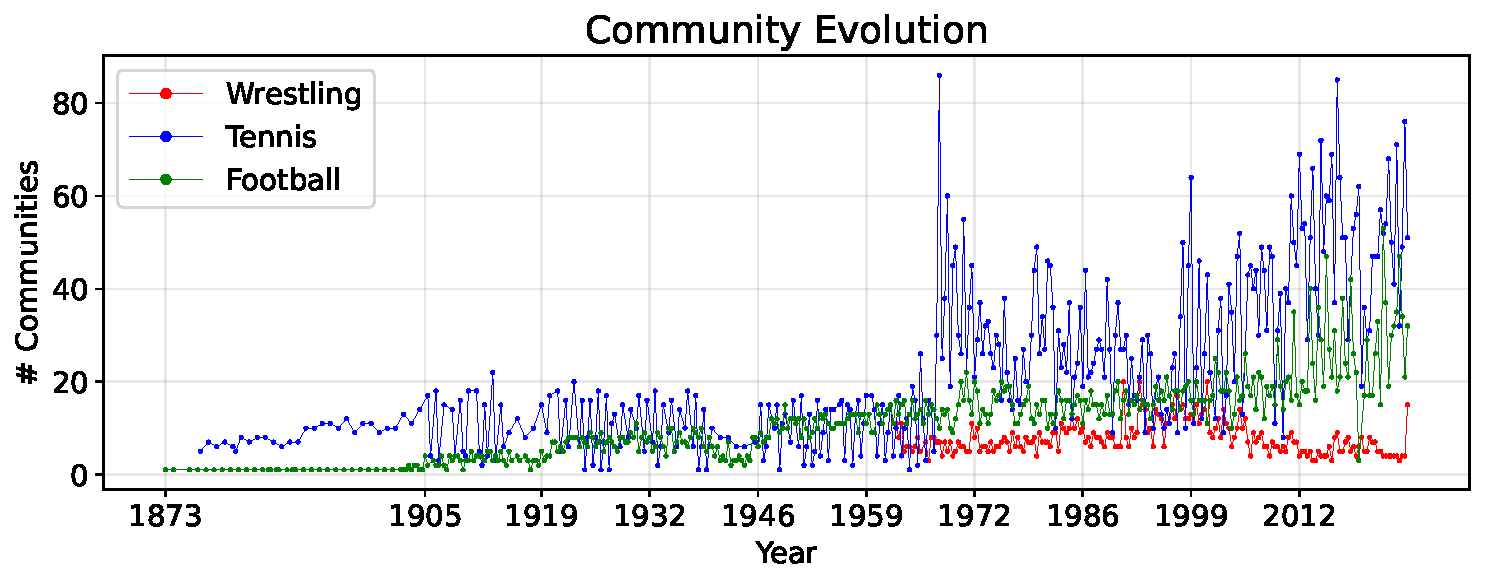
\includegraphics[width=0.8\textwidth]{plots/communities_comparison.pdf}
    \vspace{0.0cm}
    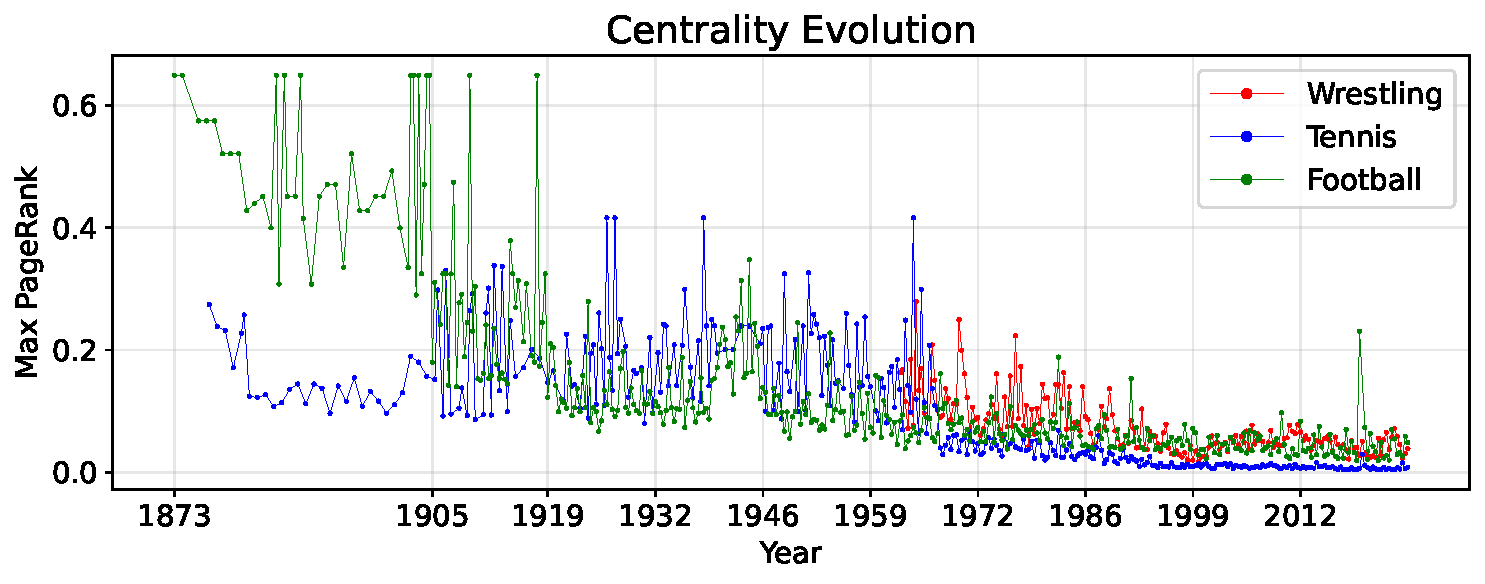
\includegraphics[width=0.8\textwidth]{plots/centrality_comparison.pdf}

    \caption{Temporal evolution comparison of density, number of communities, and centrality across Wrestling, Tennis, and Football datasets.}
    \label{fig:structural_metrics_comparison}
\end{figure}

Football shows the highest density in the early periods, followed by a strong long-term decline as the network expands and becomes sparser. Tennis exhibits a more irregular pattern, with intermittent peaks in density, especially during periods of rapid tour expansion. Wrestling remains comparatively stable and low in density, reflecting a more constrained and consistent interaction structure. Regarding community structure, tennis displays the strongest increase over time, indicating a progressively more fragmented system. Football also shows a gradual growth in the number of communities, while wrestling remains relatively stable with fewer clusters. Finally, centrality (max \texttt{PageRank}) is highest in early football and tennis periods, but decreases over time, suggesting a progressive decentralization of dominance. Wrestling maintains lower and more stable centrality values, consistent with a more evenly distributed competitive hierarchy.


\clearpage
\section{Dominance and rank evolution analysis}\label{app:dom-rank}

% WRESTLING SINGLES
\begin{figure}[!htbp]
    \centering

    \makebox[\textwidth][c]{%
        \begin{minipage}{1.18\textwidth}
            \centering
            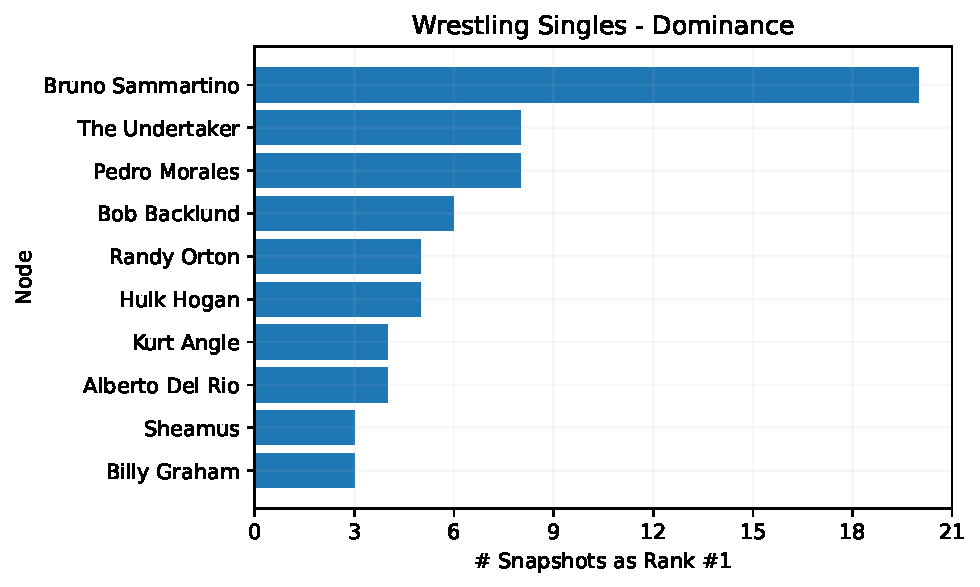
\includegraphics[width=0.39\textwidth]{plots/Wrestling Singles_dominance.pdf}
            \hspace{0.0\textwidth}
            \raisebox{0.cm}{
                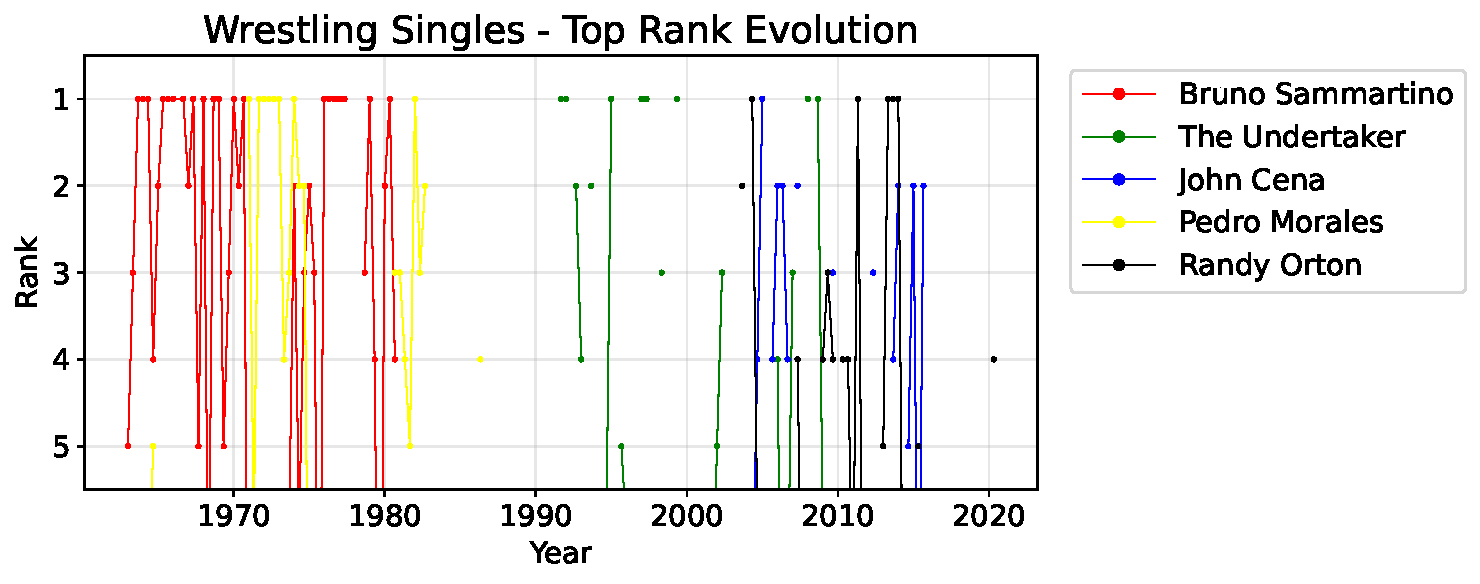
\includegraphics[width=0.58\textwidth]{plots/Wrestling Singles_rank_evolution.pdf}
            }
        \end{minipage}
    }

    \captionsetup{
        width=1.15\textwidth,
        font={footnotesize,stretch=0.9},
        labelfont=bf,
        skip=2pt
    }

    \caption{Wrestling Singles layer. Dominance score distribution (left) and temporal rank evolution (right).}
\end{figure}

% WRESTLING TAG TEAM
\begin{figure}[!htbp]
    \centering

    \makebox[\textwidth][c]{%
        \begin{minipage}{1.18\textwidth}
            \centering
            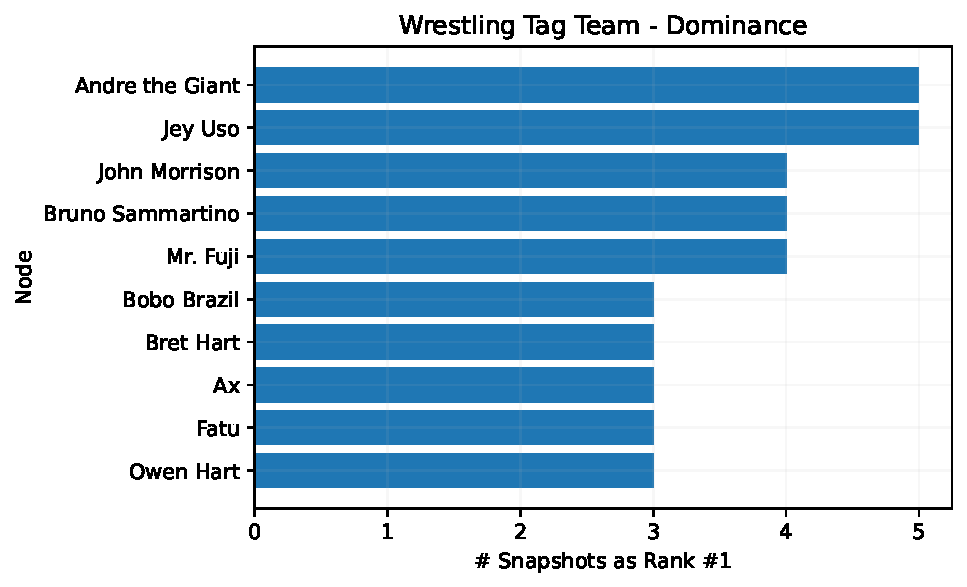
\includegraphics[width=0.39\textwidth]{plots/Wrestling Tag Team_dominance.pdf}
            \hspace{0.0\textwidth}
            \raisebox{0.cm}{
                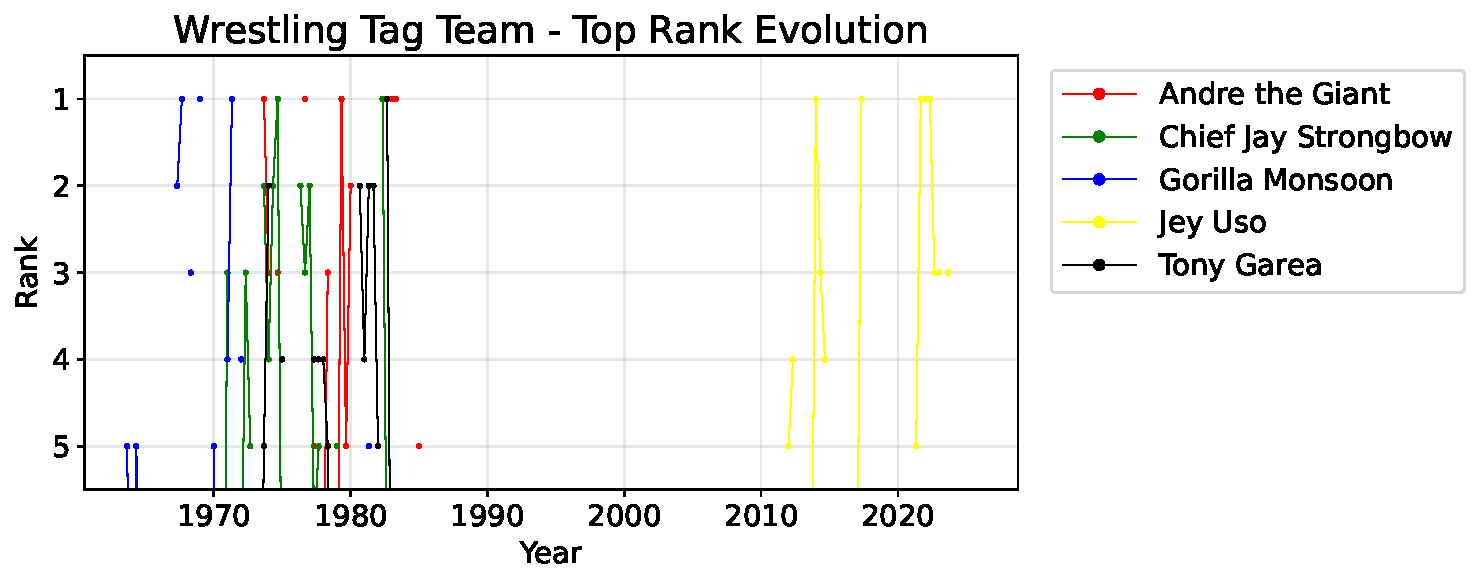
\includegraphics[width=0.58\textwidth]{plots/Wrestling Tag Team_rank_evolution.pdf}
            }
        \end{minipage}
    }

    \captionsetup{
        width=1.15\textwidth,
        font={footnotesize,stretch=0.9},
        labelfont=bf,
        skip=2pt
    }

    \caption{Wrestling Tag Team layer. Dominance score distribution (left) and temporal rank evolution (right).}
\end{figure}

% WRESTLING MULTI PERSON
\begin{figure}[!htbp]
    \centering

    \makebox[\textwidth][c]{%
        \begin{minipage}{1.18\textwidth}
            \centering
            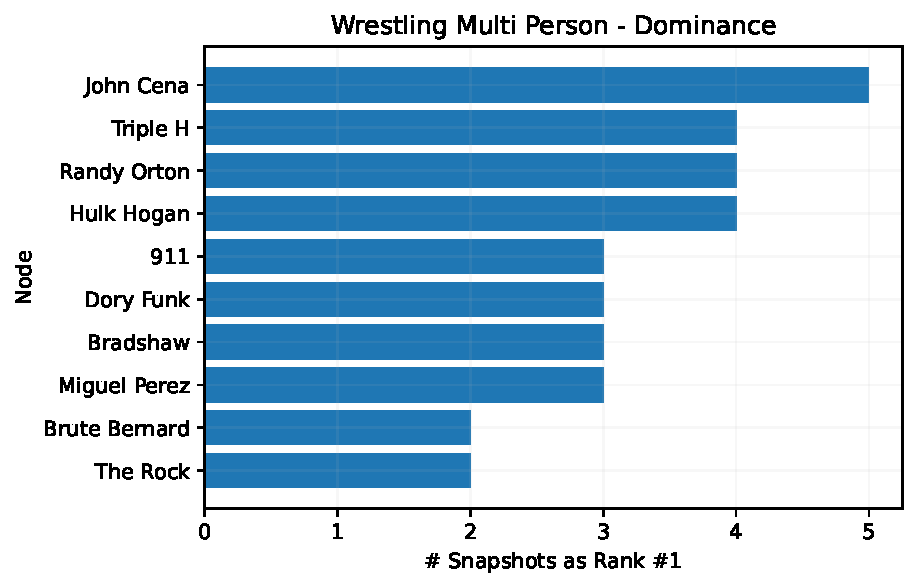
\includegraphics[width=0.39\textwidth]{plots/Wrestling Multi Person_dominance.pdf}
            \hspace{0.0\textwidth}
            \raisebox{0.cm}{
                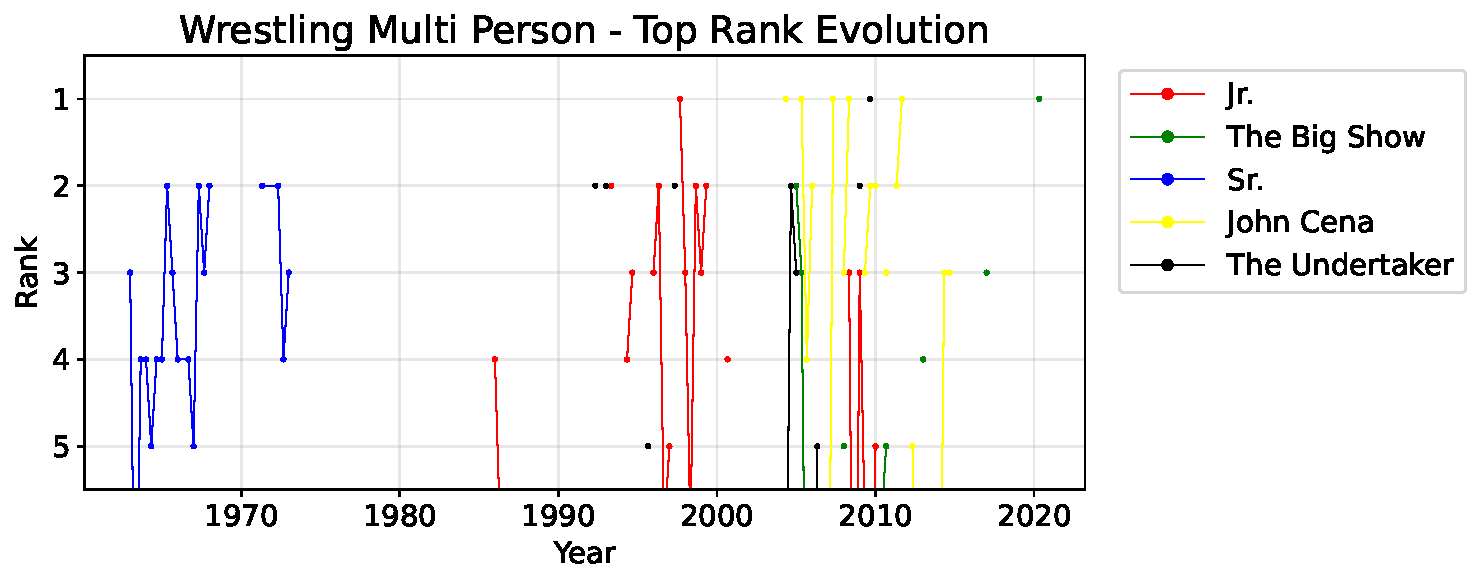
\includegraphics[width=0.58\textwidth]{plots/Wrestling Multi Person_rank_evolution.pdf}
            }
        \end{minipage}
    }

    \captionsetup{
        width=1.15\textwidth,
        font={footnotesize,stretch=0.9},
        labelfont=bf,
        skip=2pt
    }

    \caption{Wrestling Multi Person layer. Dominance score distribution (left) and temporal rank evolution (right).}
\end{figure}

% TENNIS ATP
\begin{figure}[!htbp]
    \centering

    \makebox[\textwidth][c]{%
        \begin{minipage}{1.18\textwidth}
            \centering
            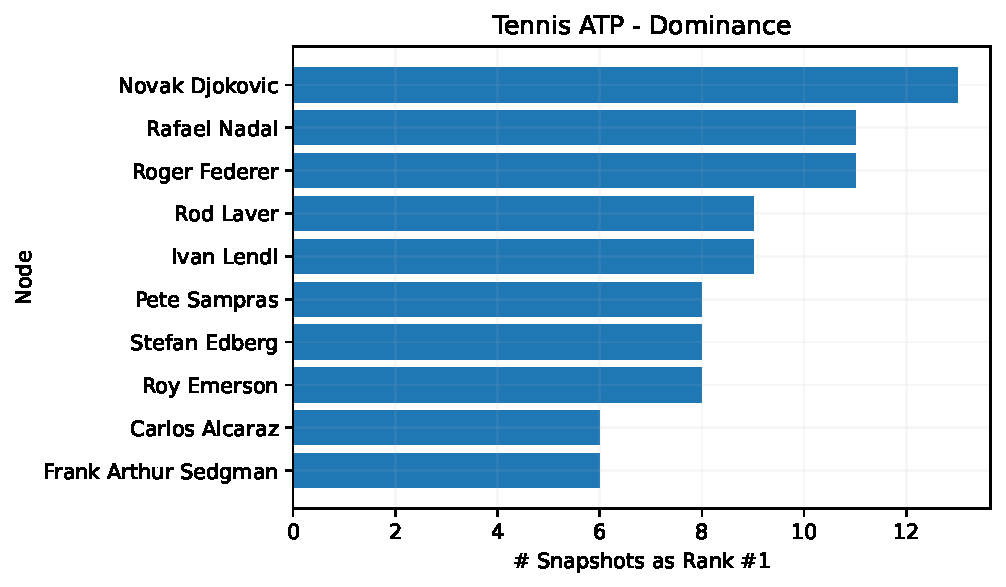
\includegraphics[width=0.39\textwidth]{plots/Tennis ATP_dominance.pdf}
            \hspace{0.0\textwidth}
            \raisebox{0.cm}{
                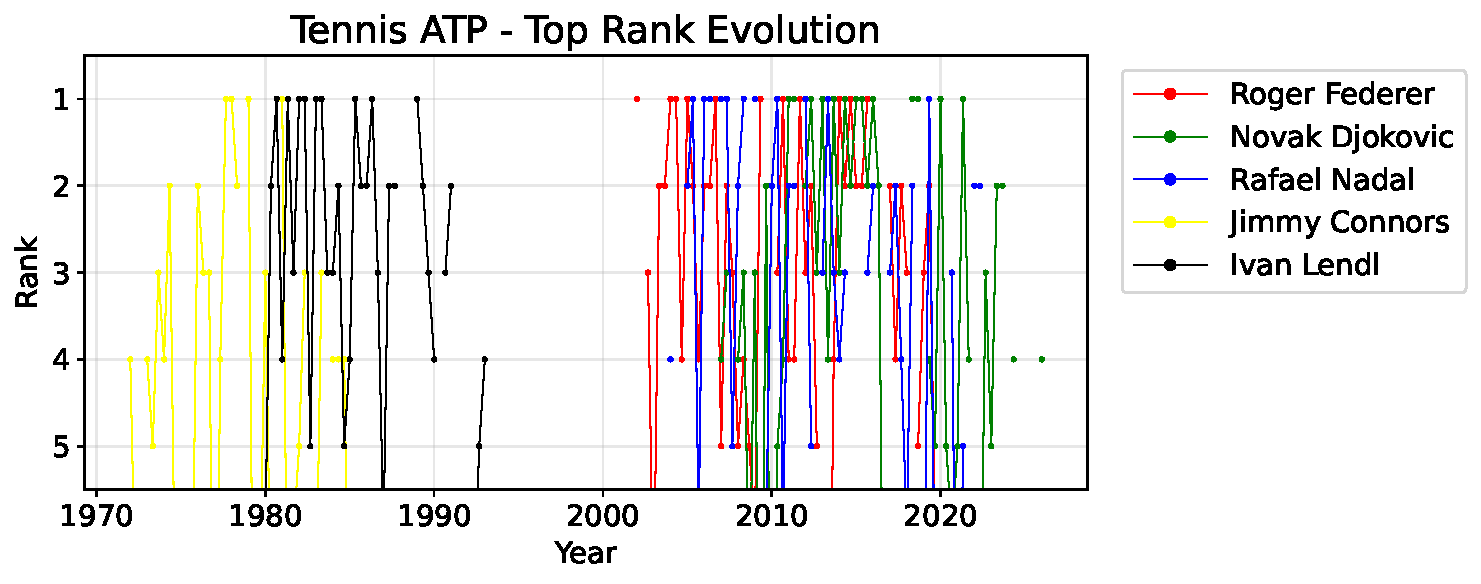
\includegraphics[width=0.58\textwidth]{plots/Tennis ATP_rank_evolution.pdf}
            }
        \end{minipage}
    }

    \captionsetup{
        width=1.15\textwidth,
        font={footnotesize,stretch=0.9},
        labelfont=bf,
        skip=2pt
    }

    \caption{ATP tennis circuit. Dominance score distribution (left) and temporal rank evolution (right).}
\end{figure}

% TENNIS WTA
\begin{figure}[!htbp]
    \centering

    \makebox[\textwidth][c]{%
        \begin{minipage}{1.18\textwidth}
            \centering
            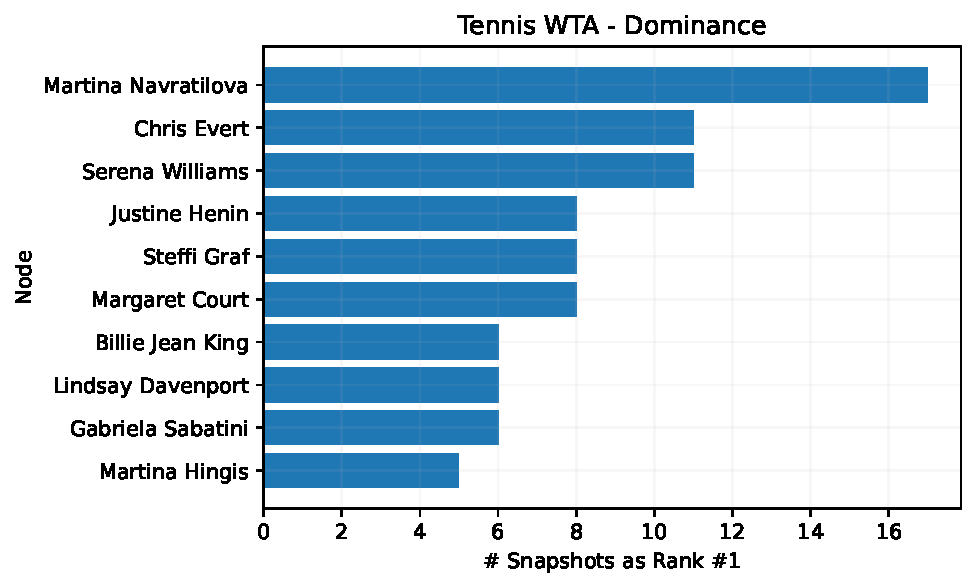
\includegraphics[width=0.39\textwidth]{plots/Tennis WTA_dominance.pdf}
            \hspace{0.0\textwidth}
            \raisebox{0.cm}{
                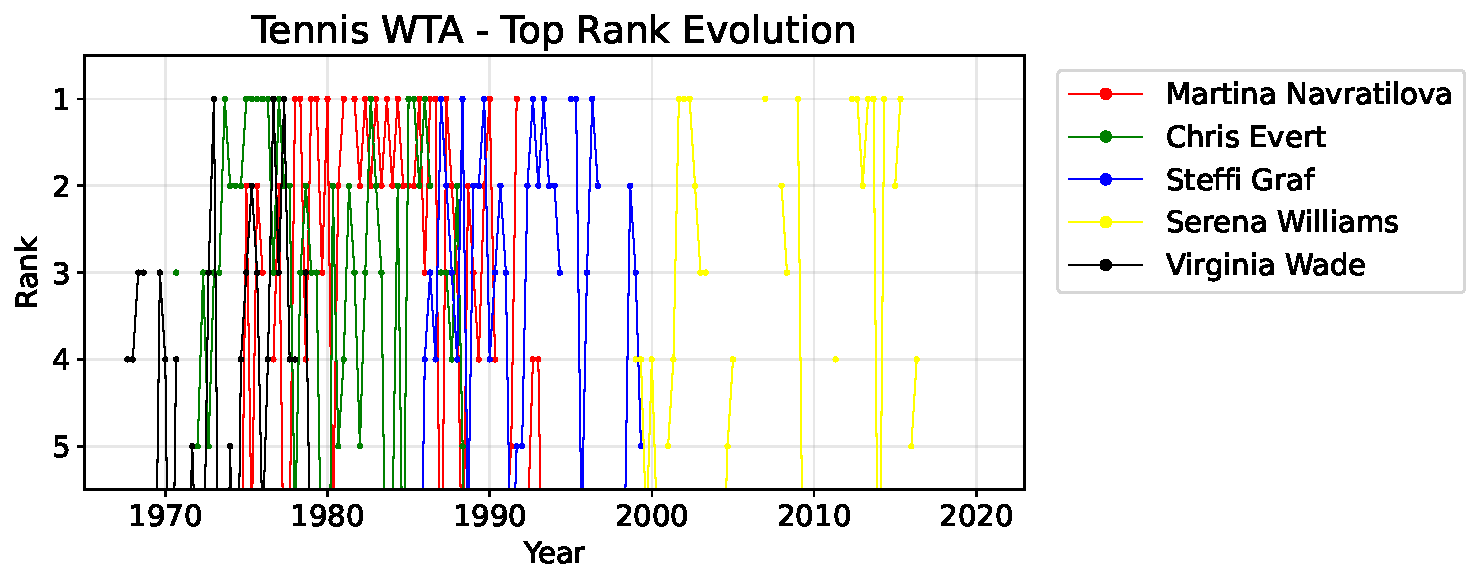
\includegraphics[width=0.58\textwidth]{plots/Tennis WTA_rank_evolution.pdf}
            }
        \end{minipage}
    }

    \captionsetup{
        width=1.15\textwidth,
        font={footnotesize,stretch=0.9},
        labelfont=bf,
        skip=2pt
    }

    \caption{WTA tennis circuit. Dominance score distribution (left) and temporal rank evolution (right).}
\end{figure}

% FIFA WORLD CUP
\begin{figure}[!htbp]
    \centering

    \makebox[\textwidth][c]{%
        \begin{minipage}{1.18\textwidth}
            \centering
            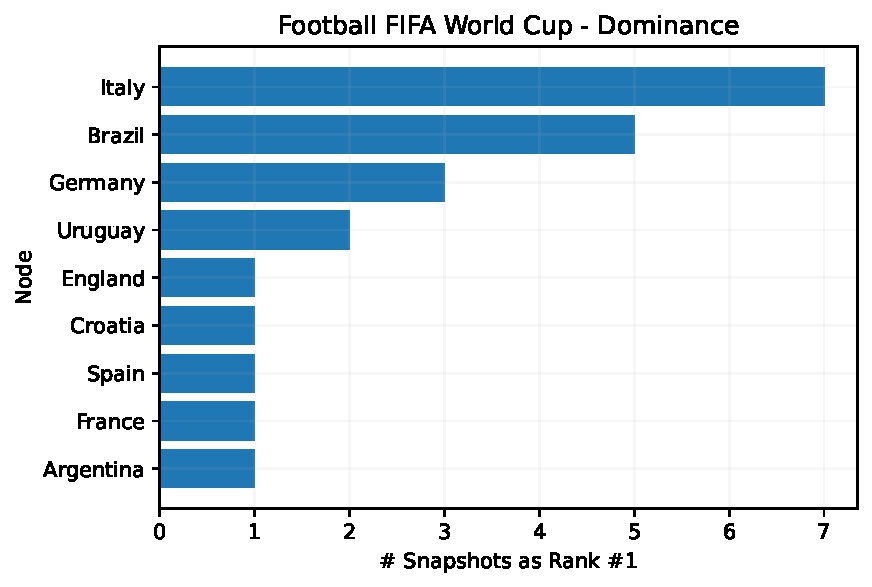
\includegraphics[width=0.39\textwidth]{plots/Football FIFA World Cup_dominance.pdf}
            \hspace{0.0\textwidth}
            \raisebox{0.3cm}{
                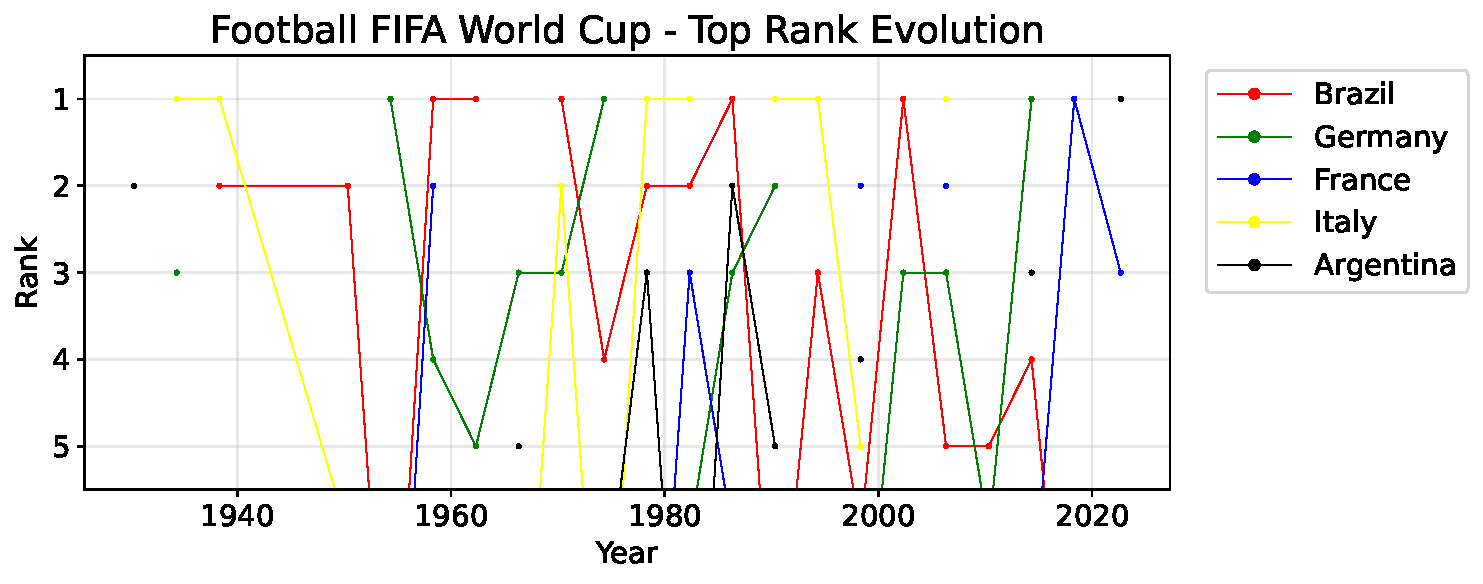
\includegraphics[width=0.58\textwidth]{plots/Football FIFA World Cup_rank_evolution.pdf}
            }
        \end{minipage}
    }

    \captionsetup{
        width=1.15\textwidth,
        font={footnotesize,stretch=0.9},
        labelfont=bf,
        skip=2pt
    }

    \caption{FIFA World Cup. Dominance score distribution (left) and temporal rank evolution (right).}
\end{figure}

% UEFA EURO
\begin{figure}[!htbp]
    \centering

    \makebox[\textwidth][c]{%
        \begin{minipage}{1.18\textwidth}
            \centering
            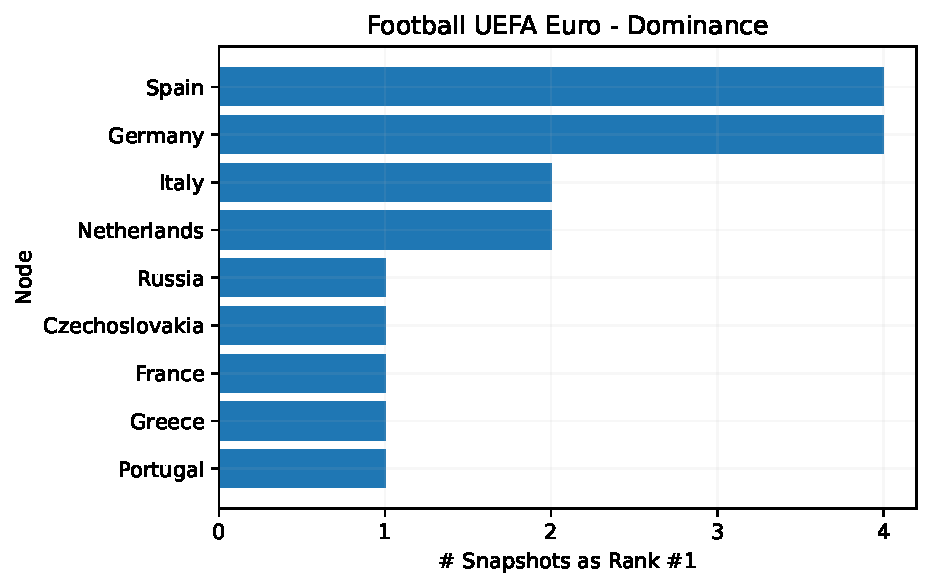
\includegraphics[width=0.39\textwidth]{plots/Football UEFA Euro_dominance.pdf}
            \hspace{0.0\textwidth}
            \raisebox{0.2cm}{
                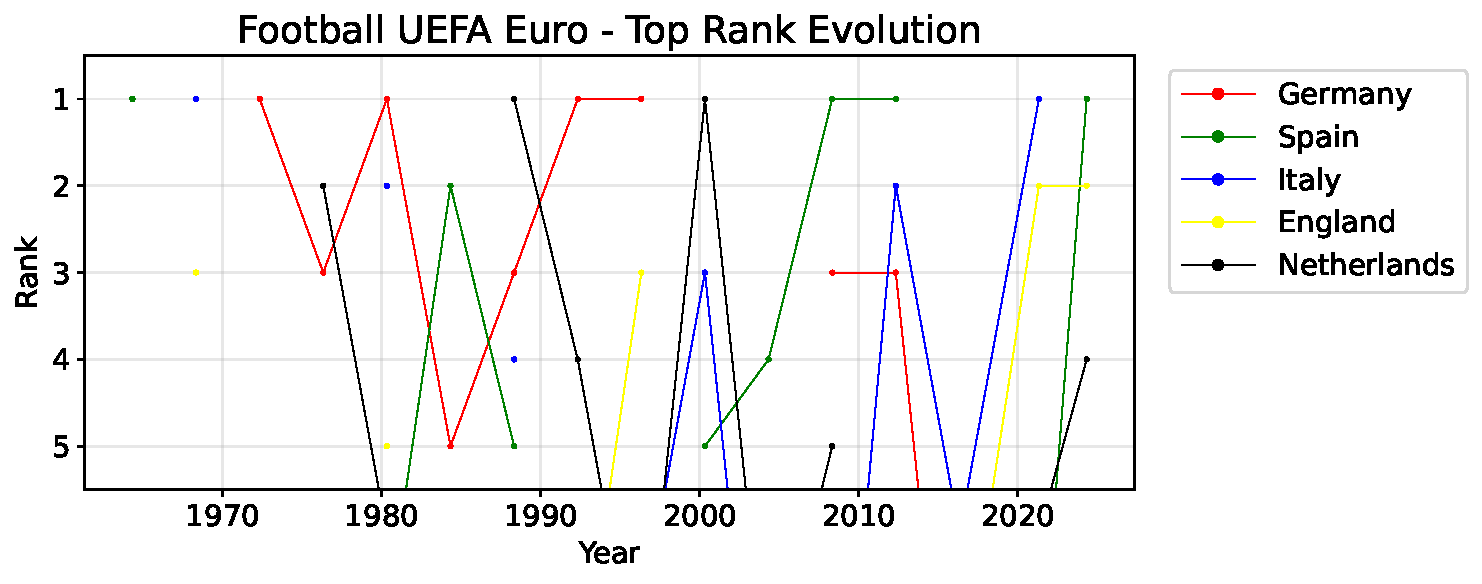
\includegraphics[width=0.58\textwidth]{plots/Football UEFA Euro_rank_evolution.pdf}
            }
        \end{minipage}
    }

    \captionsetup{
        width=1.15\textwidth,
        font={footnotesize,stretch=0.9},
        labelfont=bf,
        skip=2pt
    }

    \caption{UEFA European Championship. Dominance score distribution (left) and temporal rank evolution (right).}
\end{figure}

% =========================================================
% COPA AMERICA
% =========================================================

\begin{figure}[!htbp]
    \centering

    \makebox[\textwidth][c]{%
        \begin{minipage}{1.18\textwidth}
            \centering
            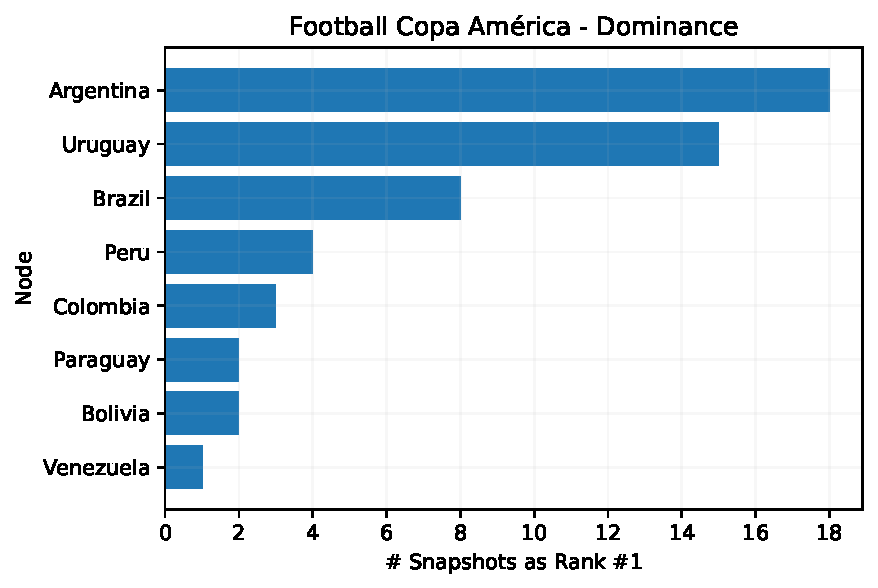
\includegraphics[width=0.39\textwidth]{plots/Football Copa América_dominance.pdf}
            \hspace{0.0\textwidth}
            \raisebox{0.3cm}{
                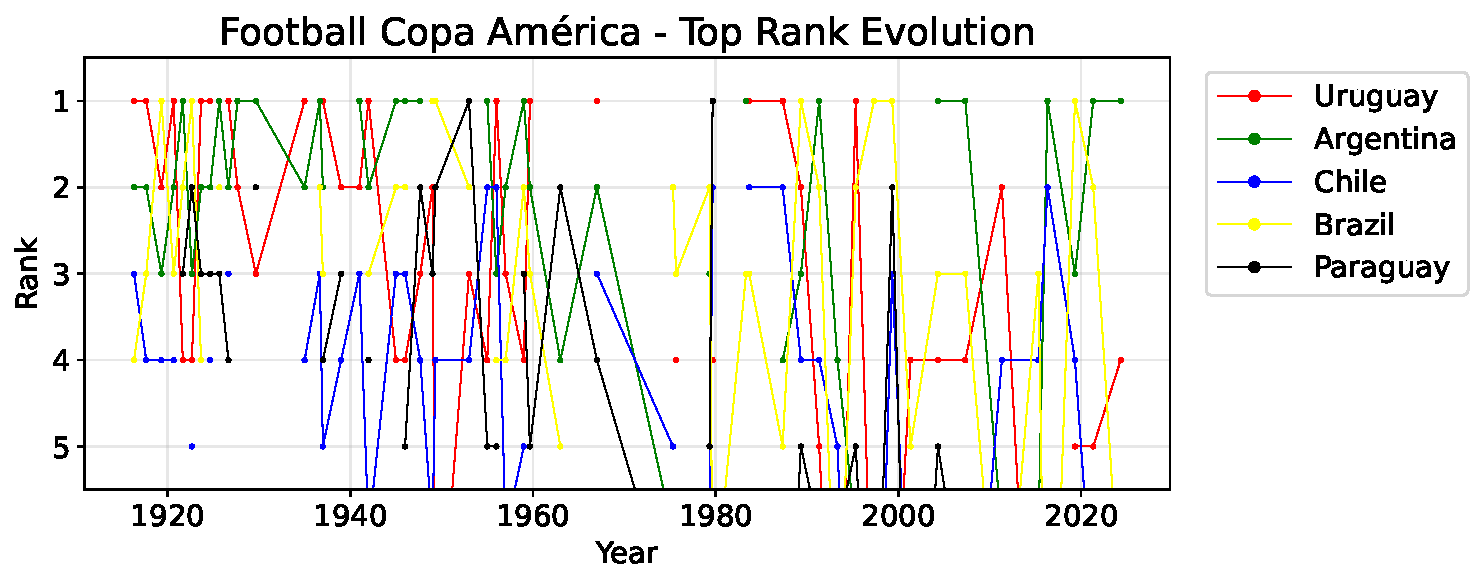
\includegraphics[width=0.58\textwidth]{plots/Football Copa América_rank_evolution.pdf}
            }
        \end{minipage}
    }

    \captionsetup{
        width=1.15\textwidth,
        font={footnotesize,stretch=0.9},
        labelfont=bf,
        skip=2pt
    }

    \caption{Copa América. Dominance score distribution (left) and temporal rank evolution (right).}
\end{figure}



\newpage